\documentclass[hyperref={bookmarks=false},aspectratio=169]{beamer}
\usepackage[utf8]{inputenc}
\usepackage{standalone}
% ---------------  Define theme and color scheme  -----------------
\usetheme[sidebarleft]{CEIT}  % 3 options: minimal, sidebarleft, sidebarright

%\setbeamertemplate{footline}[frame number]

% ------------  Information on the title page  --------------------
\title[CEIT]
{\bfseries{Centre of Excellence in IT}}

\subtitle{Premier Institute for Training and Enhancement of IT Skills}

\author[Jishnu T U] %\& Managed]
{Jishnu T U\inst{1} } %\and Managed\inst{2}}

\institute[CEIT]
{
  \inst{1}
  Trainer\\
  Centre of Excellence in IT,PNG
 % \and
 % \inst{2}
 % Trainer\\
 % Centre of Excellence in IT,PNG
}

\date[CEIT, 2014]
{Centre of Excellence in IT,PNG October 2019}
%------------------------------------------------------------

%------------------------------------------------------------
%The next block of commands puts the table of contents at the 
%beginning of each section and highlights the current section:

\AtBeginSection[]
{
  \begin{frame}
    \frametitle{Table of Contents}
    \tableofcontents[currentsection]
  \end{frame}
}

%------------------------------------------------------------


\begin{document}

\frame{\titlepage}  % Creates title page

%---------   table of contents after title page  ------------
\begin{frame}
\frametitle{Table of Contents}
\tableofcontents
\end{frame}
%---------------------------------------------------------

\section{About CEIT}

%---------------------------------------------------------
%Changing visivility of the text
\begin{frame}
\frametitle{About CEIT}
A premier institute for training and enhancement of Information Technology skills. \vspace{.4cm}
\begin{itemize}
    \item<1-> An effort of Papua New Guinea and Indian Government to create a pool of knowledge workers and generate employment opportunities by producing world class IT professional.
    \item<2-> Operated in association with University of Papua New Guinea (UPNG) and Centre for Development of Advanced Computing (C-DAC).
    \item<3-> Funded by the Government of the Republic of India in collaboration with the government of the Independent State of Papua New Guinea . 
\end{itemize}

\end{frame}


\begin{frame}
\frametitle{Vision \& Mission}
\textbf{Vision} \\
Create a pool of knowledge workers and generate employment opportunities by producing world class IT professionals.\\ \vspace{.4cm}
\textbf{Mision}
\begin{itemize}
    \item<1-> To emerge as a premier platform in Information and Communication Technologies in Papua New Guinea country for human advancement. 

    \item<2-> To generate knowledge with the dissemination of cutting edge ICT programs, for promoting professional and economic growth.

    \item<3-> To groom the students to work on current technology as well as prepare them to keep pace with the changing face of technology and the requirements of the growing IT industry.
    
    \item<4 -> To create an industry-ready talent pool to cater the Information and communications technology (ICT)
\end{itemize}

\end{frame}
\section{About UPNG}

%---------------------------------------------------------
%Changing visivility of the text
\begin{frame}
\frametitle{About UPNG}
The University of Papua New Guinea (UPNG) is a university located in Port Moresby, capital of Papua New Guinea. It was established by ordinance of the Australian administration in 1965.The UPNG offers various programs in 
 \vspace{.4cm}
\begin{itemize}
    \item Medicine \& Health Sciences, 
    \item Humanities \& Social Sciences
    \item Law
    \item Business \& Public Policy
    \item Physical \& Natural Sciences

\end{itemize}

\end{frame}
\section{About C-DAC}

%---------------------------------------------------------
%Changing visivility of the text
\begin{frame}
\frametitle{About C-DAC}
Centre for Development of Advanced Computing (C-DAC) is the premier R\&D organization of the Ministry of Electronics and Information Technology (MeitY) for carrying out R\&D in IT, Electronics and associated areas.
 \vspace{.4cm}
\begin{itemize}
    \item<1-> High Performance Computing, Multi-lingual Computing and Heritage Computing, Professional Electronics, Software Technologies, Health Informatics, Education
    \item<2-> CDAC organises courses  through the Advanced Computing Training School (ACTS) to meet the ever-increasing skilled manpower requirements of the IT industry
    \item<3-> Over the years International Cooperation Division (ICD) CDAC Delhi has progressively grown to build an eco-system and institutional framework to implementing, supervising and managing  bi-lateral projects in developing countries over more than 50 projects.
\end{itemize}

\end{frame}
\section{Certificate Courses}

%---------------------------------------------------------
%Highlighting text
\begin{frame}
\frametitle{Certificate Courses}

\begin{block}{Duration}
320 Hours
\end{block}

\begin{alertblock}{Eligibility}
Minimum of Grade 12 Certificate
\end{alertblock}


\begin{exampleblock}{Fee}
K4299 - K11299
\end{exampleblock}

\end{frame}
\section{PG Diploma Courses}

%---------------------------------------------------------
%Highlighting text
\begin{frame}
\frametitle{PG Diploma Courses}

\begin{block}{Duration}
900 Hours
\end{block}

\begin{alertblock}{Eligibility}
Bachelor in Computer Science, 
Bachelor of Information Technology, 
Bachelor of Science in Applied Physics 
Bachelor in Communication Engineering 
Bachelor of Science, Major in Mathematics, Statistics, Computer Science
Bachelor of Science, Major in Physics

\end{alertblock}


\begin{exampleblock}{Fee}
K20000
\end{exampleblock}


\end{frame}

%\begin{frame}
\frametitle{Frame Title 2}
\begin{figure}
    \centering
    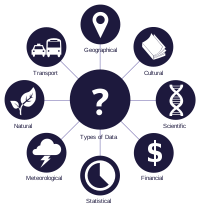
\includegraphics[width=400pt,height=210pt]{figures/fig1.png}
    \caption{``Hollywood is still mad about that, author of \emph{Legends of tech III: Techer In the Dark.}}
    \label{fig:hollywood}
\end{figure}

\end{frame}
%---------------------------------------------------------
%\section{Internet of Things}
\begin{frame}
	\frametitle{Certificate Course in Internet of Things}
	\begin{columns}
		
	\column{0.45\textwidth}
			
		\begin{figure}
			
\includegraphics[width=200pt,height=150pt]{figures/course_iot.jpg}
		\end{figure}
	
	\column{0.55\textwidth}

	\begin{block}{Description}
	
		\begin{enumerate}
			\item Embedded	Linux to develop for IoT. 
			\item Wireless Network \& Communication protocols.
			\item IoT prototyping using NodeJS and Python for development.
			\item Cloud Platforms for IoT.
		\end{enumerate}
	  	  
	\end{block}

	\end{columns}
\end{frame}








%---------------------------------------------------------

%%Two columns
\begin{frame}
\frametitle{Frame Title 4}

\begin{columns}

\column{0.45\textwidth}

\begin{figure}
    \centering
    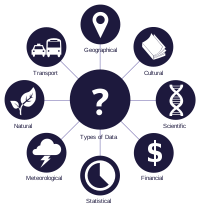
\includegraphics[scale=.4]{figures/fig1.png}
    \caption{``Hollywood is still mad about that, author of \emph{Legends of tech III: Techer In the Dark.}}
    \label{fig:hollywood_prank}
\end{figure}


\column{0.55\textwidth}
In May 1987, undergraduates from Page and Ricketts houses combined forces (and several hundred dollars) to purchase enough black and white plastic, transformed the Hollywood sign to read ``Caltech''.

\small{(Reference: http://www.admissions.caltech.edu/pranks)}

\end{columns}
\end{frame}
%---------------------------------------------------------

%---------------------------------------------------------


\end{document}